%%%%%%%%%%%%%%%%%%%%%
% Section 2         %   
% date : 17-03-2026 %
% author : fclinquart
%%%%%%%%%%%%%%%%%%%%%




\begin{frame}{Alkene's reactivity due to the $\pi$ bond}
    \begin{block}{Most reactions of alkenes involve additions to this $\pi$ bond, forming new single bonds.}
        \begin{itemize}
            \item addition with a nucleophile
            \item \textbf{addition with a radical} 
            \item Oxidation reaction 
        \end{itemize}
    \end{block}
    \begin{alertblock}{Alkenes can polymerize by Chain-reaction Polymerization \cite{de_moustier_lmapr2019_2024}}
        \begin{itemize}
            \item \textbf{Free Radical Polymerization (FRP)}
            \item \textbf{Complex coordination polymerization}
        \end{itemize}
    \end{alertblock}
\end{frame}

\begin{frame}{FRP : main reaction scheme}
    \begin{figure}
        \centering
        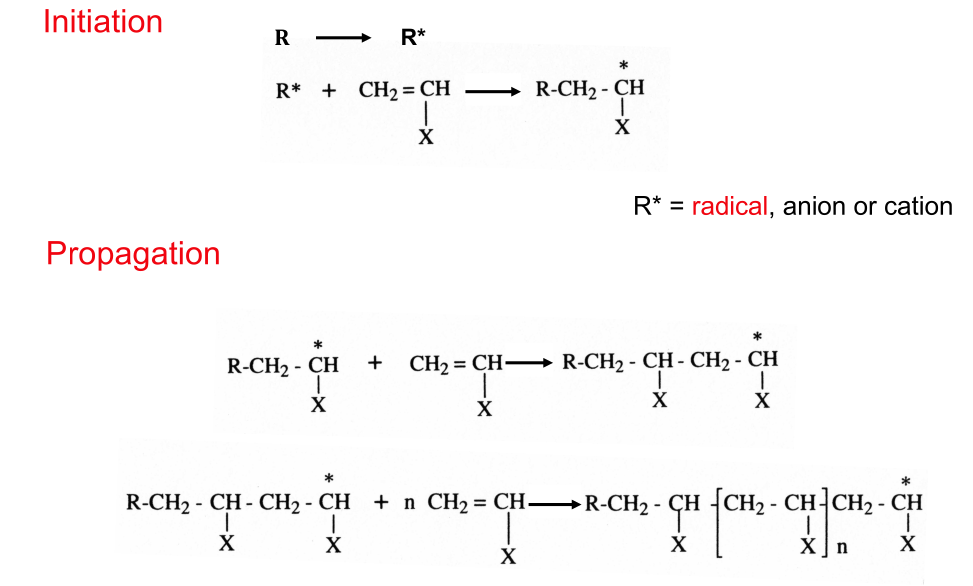
\includegraphics[width = 0.5\textwidth]{Figures/6_FRP.png}
        \caption{FRP reaction scheme.}
    \end{figure}
\end{frame}

\begin{frame}{FRP: Parameters Influencing Stereochemistry}
    Most vinyl polymers from free radical polymerization (FRP) exhibit \textbf{atacticity} due to the planar $sp^2$ radical center allowing random addition from either face  \cite{de_moustier_lmapr2019_2024}.

    Key parameters influencing stereoselectivity include:
    \begin{itemize}
        \item \textbf{Temperature}: Lower temperatures favor syndiotacticity via restricted rotation and steric control.
        \item \textbf{Steric hindrance}: Bulky R-groups increase syndiotacticity through steric hindrance.
    
    \end{itemize}
    \begin{alertblock}{PE \& PP}
    
    \textbf{PE} is not concerned. \textbf{PP} is strictly atactic in FRP
    \end{alertblock}


\end{frame}

\begin{frame}{Radical transfer between two chains lead to long branches}
    \begin{figure}
        \centering
        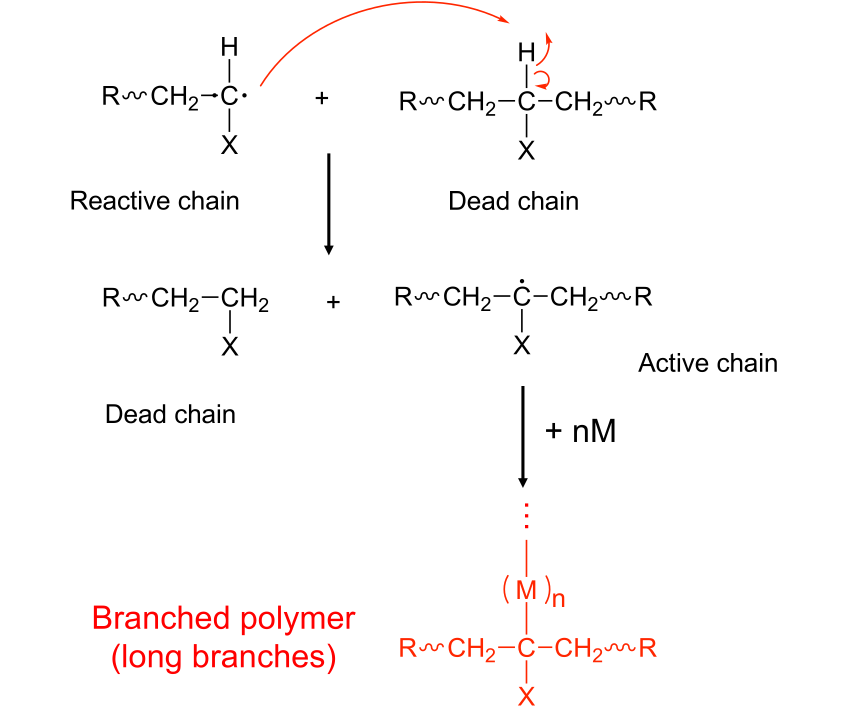
\includegraphics[width = 0.4\textwidth]{Figures/7_transfert_1.png}
        \caption{Inter-chain transfer  \cite{de_moustier_lmapr2019_2024}.}
    \end{figure}
    $\rightarrow$ long branches in PE. 
\end{frame}

\begin{frame}{Radical transfer within one chain lead to short branches}
    \begin{figure}
        \centering
        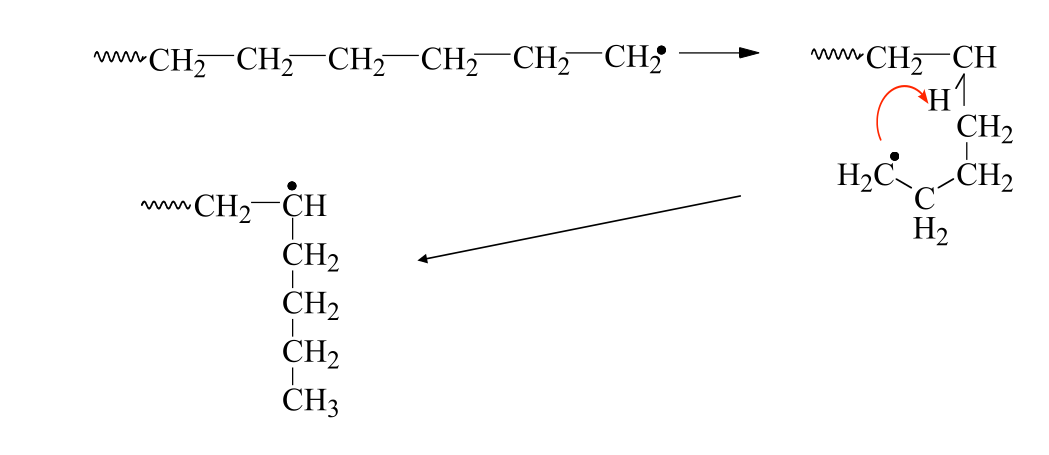
\includegraphics[width = 0.4\textwidth]{Figures/8_transfert_2.png}
        \caption{Intra-chain transfer  \cite{de_moustier_lmapr2019_2024}.}
    \end{figure}
    $\rightarrow$ short branches in PE. 
\end{frame}

\begin{frame}{Transfer to monomer}
    \begin{figure}
        \centering
        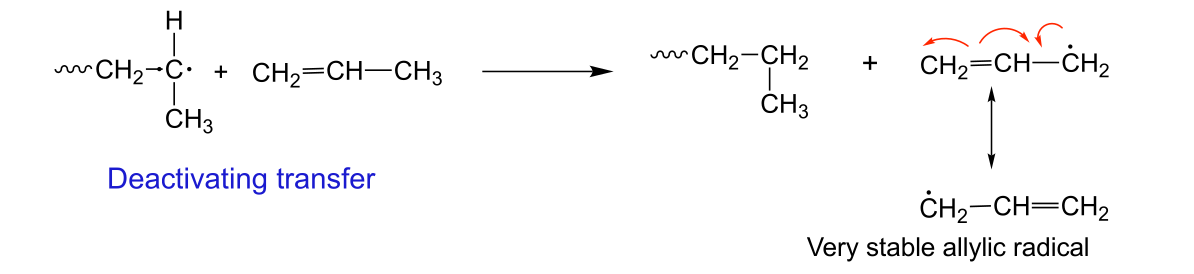
\includegraphics[width = 0.5\textwidth]{Figures/9_transfert_3.png}
        \caption{Chain neutralization in PP  \cite{de_moustier_lmapr2019_2024}.}
    \end{figure}
    $\rightarrow$ High molecular weight PP is not achievable in standard conditions.
\end{frame}

\begin{frame}{FRP : conclusion}
    \begin{minipage}{0.45\textwidth}
        \begin{block}{Only LDPE}
            \begin{itemize}
                \item High T and high P
                \item Amorphous $\leftarrow$ a lot of branches of different sizes 
                \item PDI = 7-20 
                \item Application: Soft plastic bag
            \end{itemize}
        \end{block}
    \end{minipage}
    \hfill
    \begin{minipage}{0.45\textwidth}
        \begin{block}{Only atactic PP}
            \begin{itemize}
                \item Application: Adhesive (almost never produced)
            \end{itemize}
        \end{block}
    \end{minipage}
\end{frame}

\begin{frame}{Complex coordination polymerization: a revolution}
    \begin{figure}
        \centering
        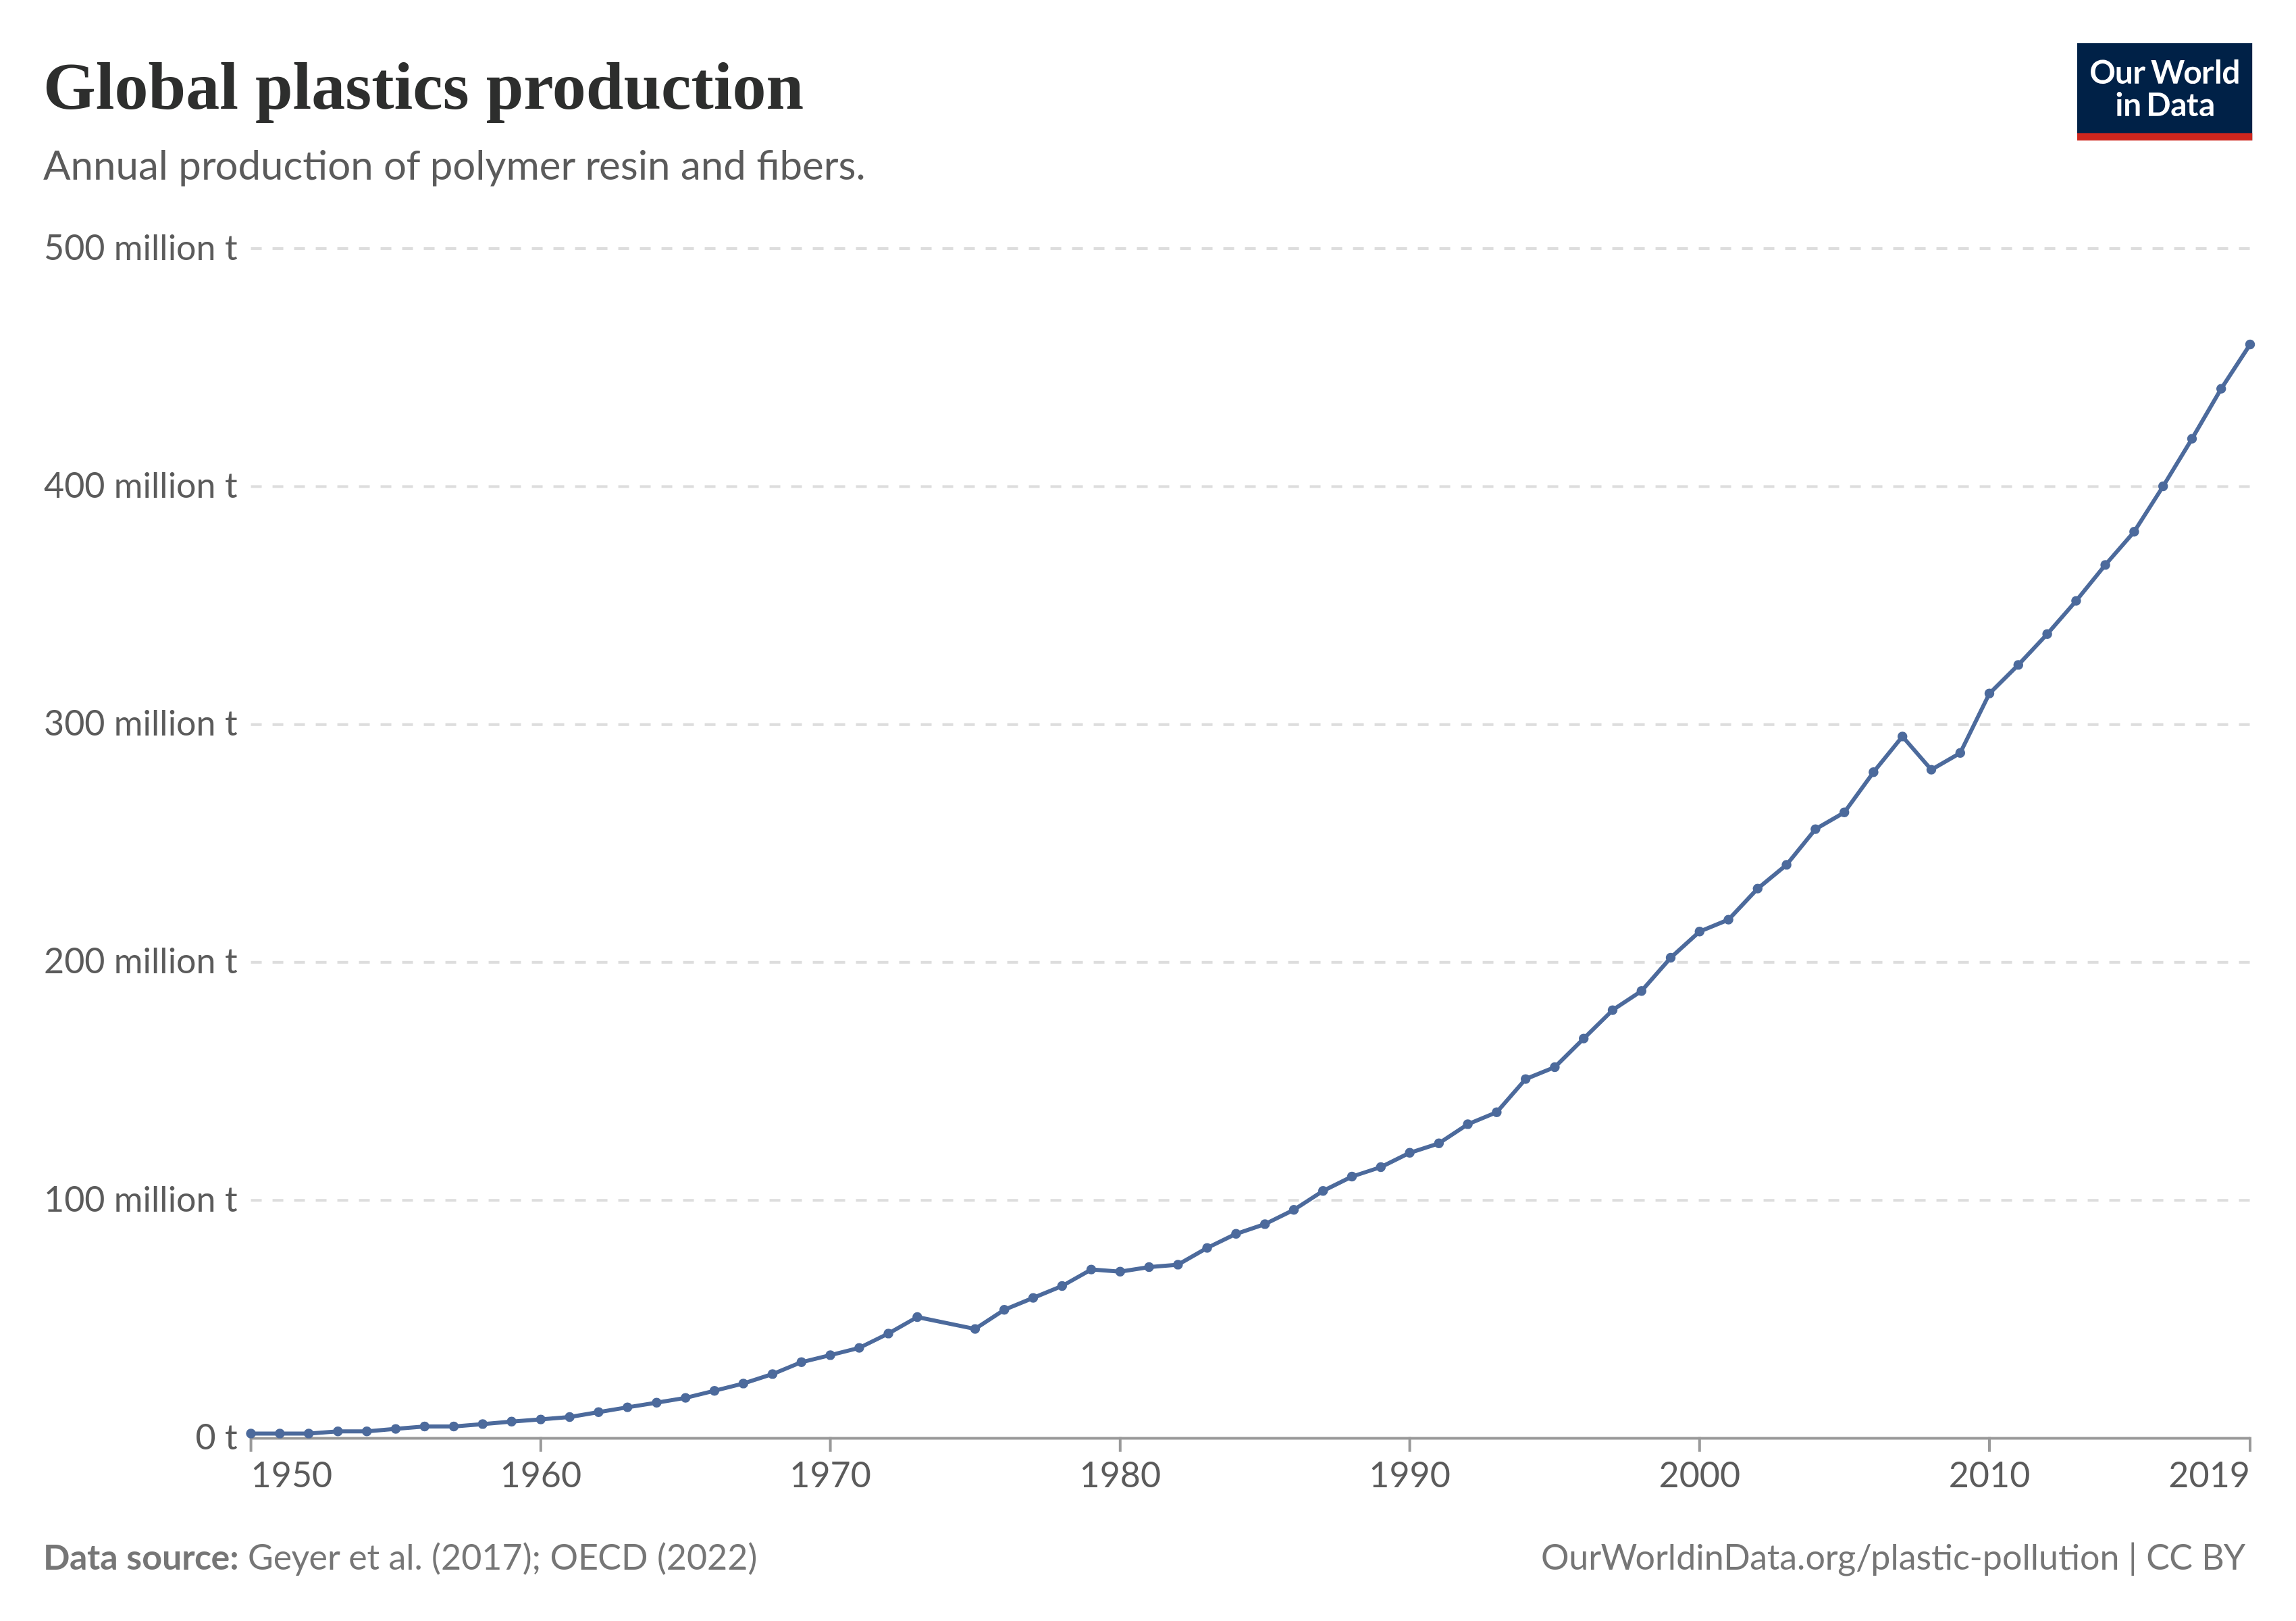
\includegraphics[width = 0.5\textwidth]{Figures/global-plastics-production.png}
        \caption{Global plastic production since 1950 \cite{owid-plastic-pollution}.}
    \end{figure}
\end{frame}

\begin{frame}{Ziegler-Natta catalyst}
    \begin{block}{Catalyst:}
        \begin{itemize}
            \item Heterogeneous transition metal (Ti)
            \item Organometallic of a metal from (I to III) (Al)
        \end{itemize}    
    \end{block}
    Typically: 
    \begin{equation}
        TiCl_4 \text{ or } TiCl_3 + AlR_3
    \end{equation}
    with \( R = CH-CH_3 \) for polyethylene. 
\end{frame}

\begin{frame}{Major results with the introduction of ZN catalyst}
    \begin{alertblock}{According to \textcite{de_moustier_lmapr2019_2024}}
        \begin{itemize}
            \item Stereospecific polymerization of PE
            \item Synthesis of linear PE
            \item Copolymerization of PP/PE
        \end{itemize}
    \end{alertblock}
    $\rightarrow$ Control of stereoregularity/stereochemistry and \( M_w \) through termination reactions. 
    $\rightarrow$ Tacticity depends on the crystalline form of the catalyst. 
\end{frame}

\begin{frame}{Major Polyolefins made by ZN catalyst}
    \begin{minipage}{0.45\textwidth}
        \begin{block}{PE}
            \begin{itemize}
                \item HDPE ($\xi_c = 0.9$ \& PDI = 3-5)
                \item UHWPE ($M_w = \pm 3 \times 10^6$)
                \item LLDPE (Ethylene copolymer with 5-12\% of $\alpha$-olefin)
            \end{itemize}
        \end{block}
    \end{minipage}
    \hfill
    \begin{minipage}{0.45\textwidth}
        \begin{block}{Isotactic PP}
            \begin{itemize}
                \item Soluble metallocene catalyst
                \item 99\% tacticity 
            \end{itemize}
        \end{block}
    \end{minipage}
\end{frame}

